% Chapter 2: Requirements Specification, Analysis, and Architecture

\chapter{Requirements Specification, Analysis, and Architecture}
\label{ch:chapter2}

\section{Introduction}
This chapter specifies the requirements, threat boundaries, and structural architecture of the secure platform. By mapping actors, defining functional security parameters, establishing non-functional cryptographic requirements, detailing a security-oriented product backlog, and detailing our Zero-Knowledge architecture, we lay the engineering specifications for the application.

\section{Needs Analysis and Specification}
To secure the collaboration space, the analysis separates cryptographic operations from generic data transport.

\subsection{Identification of Actors}
To align with our UML Use Case analysis and role-based access control, we identify several distinct human actors based on their privileges, alongside our central system actor:
\begin{itemize}
    \item \textbf{Unregistered User}: A guest actor whose only capabilities are registering a new account or authenticating an existing session.
    \item \textbf{Authenticated User}: A logged-in user who can manage their global profile settings, switch interface themes, join existing servers via invite links, or create entirely new servers.
    \item \textbf{Server Member}: An authenticated user who has joined a specific server. This actor can participate in real-time text channels, share files, and establish peer-to-peer WebRTC connections in voice channels.
    \item \textbf{Server Owner}: A privileged server member with elevated administrative rights. This actor is responsible for generating invite links, provisioning new text or voice channels, and managing role delegations.
\end{itemize}

\subsection{Capture of Functional Requirements}
The functional requirements of the system are categorized based on the capabilities granted to each specific actor:
\begin{itemize}
    \item \textbf{Unregistered User Requirements}: The system must allow guest users to register a new account using an email and password, and authenticate existing sessions securely to obtain an access token.
    \item \textbf{Authenticated User Requirements}: The system must allow logged-in users to manage their profile (e.g., update display name), toggle UI preferences like dark mode, create new personal servers, and join existing servers using valid invite links.
    \item \textbf{Server Member Requirements}: The system must enable members to participate in real-time text channels (send, edit, delete messages, and upload files), receive @mention notifications, and establish peer-to-peer WebRTC connections in voice channels with the ability to mute, deafen, or share screens.
    \item \textbf{Server Owner Requirements}: The system must provide elevated administrative controls allowing owners to generate and revoke invite links, provision new text and voice channels, create custom roles with specific permissions, assign roles to members, and perform moderation actions (kick, ban, timeout).
\end{itemize}

\subsection{Analysis of Non-Functional Requirements}
Non-functional requirements define how the system should perform rather than what it does. For our application, we focus on providing a smooth and reliable user experience:
\begin{itemize}
    \item \textbf{Real-Time Performance}: The system must deliver text messages and voice audio instantly with minimal delay, ensuring conversations feel natural and responsive.
    \item \textbf{Usability and User Experience}: The application interface must be intuitive, visually appealing, and easy to navigate for non-technical users. Features like Dark Mode should be included to improve visual comfort.
    \item \textbf{Scalability}: The backend server must be capable of handling multiple active users, servers, and voice channels simultaneously without crashing or slowing down.
    \item \textbf{Standard Security and Privacy}: User passwords must be safely hashed before being stored in the database, and user sessions must be secured using authentication tokens to prevent unauthorized access.
\end{itemize}

\begin{figure}[H]
    \centering
    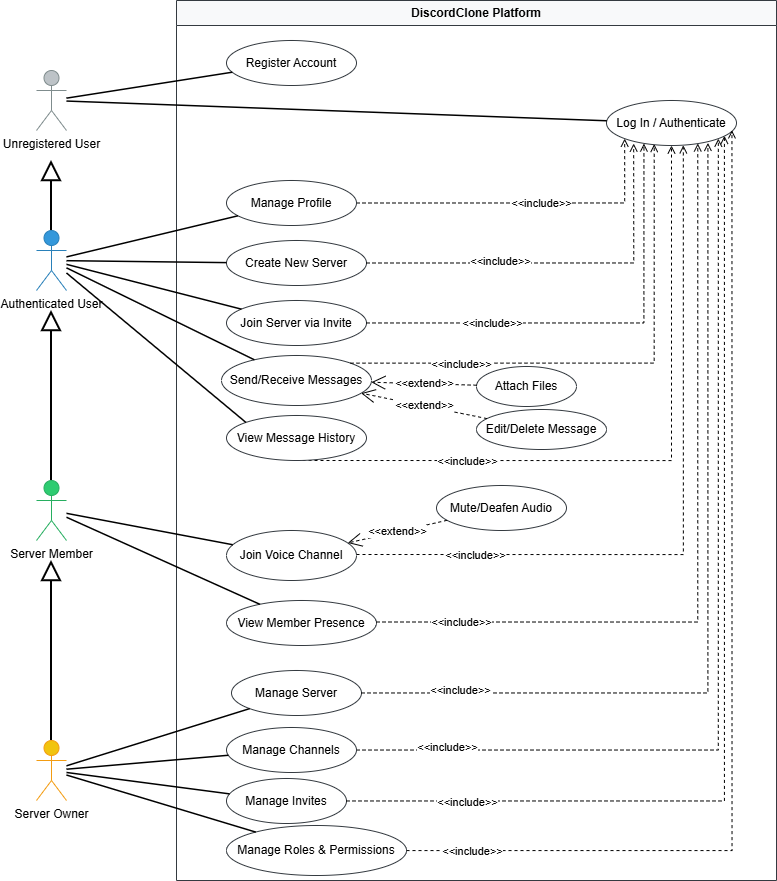
\includegraphics[width=0.9\textwidth]{use_case_diagram.png}
    \caption{Global UML Use Case Diagram of the DiscordClone Platform.}
    \label{fig:use_case_diagram}
\end{figure}

\section{Product Backlog}
The global product backlog is organized into five sprints, prioritizing features by security boundaries, real-time communications, and deployment needs. This comprehensive roadmap guides the implementation process:

% CHANGED: Adjusted column widths to fix overflows
\small
\begin{longtable}{| p{1.2cm} | p{1.8cm} | p{10.0cm} | p{1.8cm} | p{1.2cm} |}
    \hline
    \rowcolor{lightgray}
    \textbf{ID} & \textbf{Sprint} & \textbf{User Story Description} & \textbf{Priority} & \textbf{Points} \\
    \hline
    \endfirsthead
    \hline
    \rowcolor{lightgray}
    \textbf{ID} & \textbf{Sprint} & \textbf{User Story Description} & \textbf{Priority} & \textbf{Points} \\
    \hline
    \endhead
    \hline
    \endfoot
    \hline
    \endlastfoot
    
    S1-01 & Sprint 1 & As a new user, I want to register an account with my email and a password, so that I can access the platform. & P0 & 3 \\
    \hline
    S1-02 & Sprint 1 & As a registered user, I want to log in with my email and password, so that I can access my account and servers. & P0 & 3 \\
    \hline
    S1-03 & Sprint 1 & As a logged-in user, I want to log out of my account, so that my session ends and no one else can use my account. & P1 & 1 \\
    \hline
    S1-04 & Sprint 1 & As a logged-in user, I want to view and edit my display name, so that other users see the name I choose. & P1 & 2 \\
    \hline
    S2-01 & Sprint 2 & As a user, I want to create a new server, so that I have a private space to invite my friends. & P0 & 3 \\
    \hline
    S2-02 & Sprint 2 & As a server owner, I want to generate an invite link for my server, so that I can share it with friends so they can join. & P0 & 3 \\
    \hline
    S2-03 & Sprint 2 & As a user, I want to join a server using an invite link, so that I can participate in that community. & P0 & 2 \\
    \hline
    S2-04 & Sprint 2 & As a server owner, I want to create text and voice channels inside my server, so that I can organize conversations by topic. & P1 & 3 \\
    \hline
    S2-05 & Sprint 2 & As a server owner, I want to create roles and assign them to members, so that I can delegate responsibilities and control who can do what. & P1 & 5 \\
    \hline
    S2-06 & Sprint 2 & As a server member, I want to leave a server I no longer want to be part of, so that I am not in servers that are no longer relevant to me. & P2 & 2 \\
    \hline
    S3-01 & Sprint 3 & As a server member, I want to send a message in a text channel and have everyone see it instantly, so that we can have a real-time conversation. & P0 & 8 \\
    \hline
    S3-02 & Sprint 3 & As a server member, I want to see recent messages when I open a channel, so that I can catch up on what was discussed before I arrived. & P1 & 3 \\
    \hline
    S3-03 & Sprint 3 & As a server member, I want to see which members of a server are online or offline, so that I know who is available to chat. & P1 & 3 \\
    \hline
    S3-04 & Sprint 3 & As a server member, I want to edit my own messages after sending them, so that I can fix mistakes. & P1 & 2 \\
    \hline
    S3-05 & Sprint 3 & As a server member, I want to delete my own messages, so that I can remove something I no longer want to have posted. & P1 & 2 \\
    \hline
    S4-01 & Sprint 4 & As a server member, I want to join a voice channel and talk with others in real time, so that we can have live voice conversations. & P0 & 8 \\
    \hline
    S4-02 & Sprint 4 & As a voice channel participant, I want to mute my microphone, so that I can stop broadcasting audio without leaving the channel. & P1 & 2 \\
    \hline
    S4-03 & Sprint 4 & As a voice channel participant, I want to deafen myself, so that I can stop hearing others without leaving the channel. & P1 & 2 \\
    \hline
    S4-04 & Sprint 4 & As a voice channel participant, I want to see who is currently in the voice channel, so that I can follow the conversation and know who is present. & P1 & 3 \\
    \hline
    S4-05 & Sprint 4 & As a voice channel participant, I want to leave the voice channel, so that I stop being part of the voice call. & P1 & 1 \\
    \hline
    EXT-01 & Extended & As a server member, I want to attach an image or a file to a message, so that I can share content with other members. & P1 & 5 \\
    \hline
    EXT-02 & Extended & As a user, I want to switch to a dark mode interface, so that the app is comfortable to use at night. & P2 & 2 \\
    \hline
    EXT-03 & Extended & As a server member, I want to receive a notification when I am mentioned in a message, so that I do not miss messages addressed to me. & P2 & 3 \\
    \hline
    \caption{\textbf{Global Unified Product Backlog.}}
    \label{tab:global_backlog} \\
\end{longtable}
\normalsize

\section{Release Planning}
In this section, we planned the releases of our application using the created backlog. Each release has its own sprints, and each sprint has its own backlog containing several user stories from the initial backlog. During each sprint, we proceeded with the design and implementation of the assigned functionalities and concluded with an evaluation. The figure below presents our release planning.

\begin{figure}[H]
    \centering
    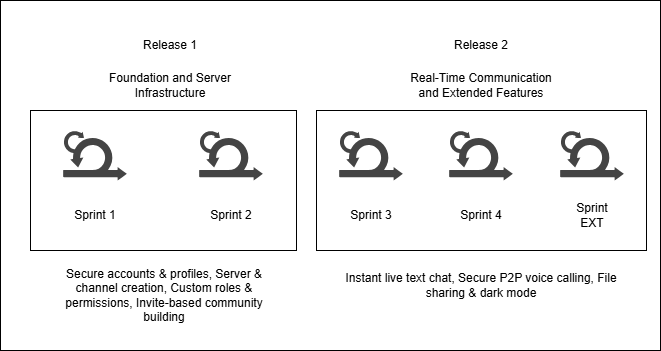
\includegraphics[width=0.85\textwidth]{release_planning.png}
    \caption{Release Planning: Sprint Distribution across Releases.}
    \label{fig:release_planning}
\end{figure}

\section{Work Environment}
This section is dedicated to presenting the technologies used in the development and architecture of our application, as well as the complementary technologies leveraged during the realization of our project.

\subsection{Development Technologies}
To satisfy these strict security objectives, our development environment is configured with optimized real-time and cryptographic engines:

\subsection*{Database}
\noindent
\begin{minipage}[t]{1.5cm}
    \vspace{0pt}
    \includegraphics[width=1.5cm]{postgres.png}
\end{minipage}%
\hspace{0.3cm}
\begin{minipage}[t]{\dimexpr\textwidth-1.9cm\relax}
    \vspace{0pt}
    \small
    \textbf{PostgreSQL} is our chosen database management system (specifically hosted via Neon). This robust relational system is configured for optimal performance and strict constraints to handle our Zero-Knowledge storage schemas effectively.
\end{minipage}
\vspace{0.3cm}

\subsection*{Backend Server}
\noindent
\begin{minipage}[t]{1.5cm}
    \vspace{0pt}
    
\includegraphics[width=1.5cm]{spring_boot.png}
\end{minipage}%
\hspace{0.3cm}
\begin{minipage}[t]{\dimexpr\textwidth-1.9cm\relax}
    \vspace{0pt}
    \small
    \textbf{Spring Boot 4.0.3 (Java 21)} is used to build our neutral signaling backend, managed via \textbf{Maven}. It exposes a RESTful API integrated with robust WebSocket support for real-time messaging. Key backend libraries and configurations include:
    \begin{itemize}
        \item \textbf{Security}: Implemented using Spring Security and JWT (via the JJWT library) to authenticate users securely.
        \item \textbf{Spring Data JPA}: Used as the Object-Relational Mapping (ORM) layer to interact with the PostgreSQL database.
        \item \textbf{Spring WebSocket}: Coordinates real-time messaging and WebRTC signaling over stateful connection channels.
        \item \textbf{Jackson}: Handles reliable JSON serialization and deserialization across the network.
    \end{itemize}
\end{minipage}
\vspace{0.3cm}

\subsection*{Frontend Client}
\noindent
\begin{minipage}[t]{1.5cm}
    \vspace{0pt}
    
\includegraphics[width=1.5cm]{nextjs.png}
\end{minipage}%
\hspace{0.3cm}
\begin{minipage}[t]{\dimexpr\textwidth-1.9cm\relax}
    \vspace{0pt}
    \small
    \textbf{Next.js 16.1.7} is used to build our client application. This framework renders our dynamic UI while handling client-side cryptography via the high-performance WebCrypto API and the robust libsodium library. Furthermore, it manages direct multi-peer real-time audio streams routed using WebRTC P2P connection channels.
\end{minipage}
\vspace{0.3cm}

\subsection{Complementary Technologies}
These are the technologies that were leveraged during the realization of our project:

\subsection*{IntelliJ IDEA}
\noindent
\begin{minipage}[t]{1.5cm}
    \vspace{0pt}
    \includegraphics[width=1.5cm]{intellij.png}
\end{minipage}%
\hspace{0.3cm}
\begin{minipage}[t]{\dimexpr\textwidth-1.9cm\relax}
    \vspace{0pt}
    \small
    \textbf{IntelliJ IDEA} is a powerful Integrated Development Environment (IDE) tailored for Java development. It significantly accelerates backend development with Spring Boot by providing advanced code assistance, seamless Maven integration, and deep analytical debugging.
\end{minipage}
\vspace{0.3cm}

\subsection*{Postman}
\noindent
\begin{minipage}[t]{1.5cm}
    \vspace{0pt}
    \includegraphics[width=1.5cm]{postman.png}
\end{minipage}%
\hspace{0.3cm}
\begin{minipage}[t]{\dimexpr\textwidth-1.9cm\relax}
    \vspace{0pt}
    \small
    \textbf{Postman} is a collaboration platform for API development. It allows for the efficient creation, testing, and debugging of our REST endpoints, ensuring that the backend services integrate properly with the client application.
\end{minipage}
\vspace{0.3cm}

\subsection*{Draw.io}
\noindent
\begin{minipage}[t]{1.5cm}
    \vspace{0pt}
    
\includegraphics[width=1.5cm]{drawio.png}
\end{minipage}%
\hspace{0.3cm}
\begin{minipage}[t]{\dimexpr\textwidth-1.9cm\relax}
    \vspace{0pt}
    \small
    \textbf{Draw.io} is a versatile diagramming application used to construct the structural and dynamic models of the application, such as UML Class Diagrams, Sequence Diagrams, and Physical Deployment Diagrams.
\end{minipage}
\vspace{0.3cm}

\subsection*{PlantUML}
\noindent
\begin{minipage}[t]{1.5cm}
    \vspace{0pt}
    
\includegraphics[width=1.5cm]{plantuml.png}
\end{minipage}%
\hspace{0.3cm}
\begin{minipage}[t]{\dimexpr\textwidth-1.9cm\relax}
    \vspace{0pt}
    \small
    \textbf{PlantUML} is an open-source tool that lets you create diagrams by writing text code instead of drawing shapes manually. It supports various chart types—from standard UML (like Sequence or Class diagrams) to Mind maps and Gantt charts. This text-based approach makes diagrams easy to edit and version-controlled alongside your code.
\end{minipage}
\vspace{0.3cm}

\subsection*{pgAdmin}
\noindent
\begin{minipage}[t]{1.5cm}
    \vspace{0pt}
    
\includegraphics[width=1.5cm]{pgadmin.png}
\end{minipage}%
\hspace{0.3cm}
\begin{minipage}[t]{\dimexpr\textwidth-1.9cm\relax}
    \vspace{0pt}
    \small
    \textbf{pgAdmin} is the leading open-source administration and development platform for PostgreSQL. It was utilized to securely monitor database schemas, execute queries, and manage the underlying persistence layer of our architecture.
\end{minipage}
\vspace{0.3cm}


\subsection{Version Control}
For the version control of our project, we used Git and GitHub to manage collaborative work and track modifications. To maintain a structured and reliable codebase, we adopted a strict branching strategy. The \textbf{main} branch served as the stable core of our project. Whenever we needed to implement new functionality, we branched out into dedicated feature branches. Once the new features were fully developed and tested, we merged them back into the \textbf{main} branch to ensure seamless integration.

\begin{figure}[H]
    \centering
    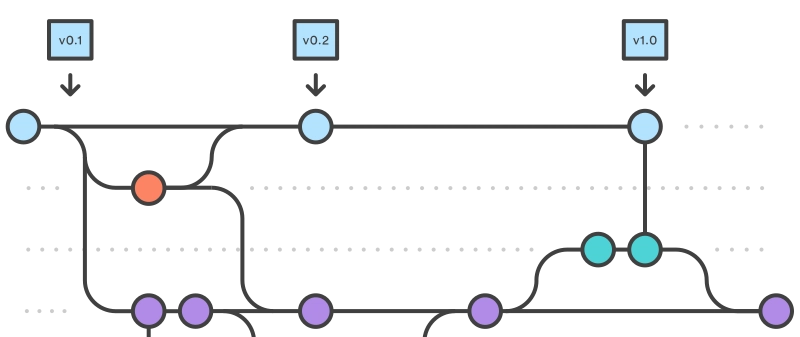
\includegraphics[width=1\textwidth]{git_branching.png}
    \caption{Git Branching and Merging Strategy Model.}
    \label{fig:git_branching}
\end{figure}

\section{Architectural Model}
Early on in the development process, the application architecture is established. It lays out the road map and best practices to adhere to in creating an organized application.

We designed a Zero-Knowledge architecture that prevents server-side access to plaintext data.

\subsection{Logical Architecture}
The choice of our system's architecture is a very important step. It is often dictated by the technical needs of our application in terms of organization and development, as well as maintenance requirements. In this context, the MVC (Model-View-Controller) architecture proves highly effective, hence our choice of the MVC architecture model presented below.

This architecture consists of separating the application components into three distinct parts: the model, the view, and the controller:
\begin{itemize}
    \item \textbf{Model}: This part of the architecture contains the application data, structured as entities using the concept of object-relational mapping. This layer interacts directly with the database.
    \item \textbf{Controller}: Located between the model and the view, this layer receives user requests, determines the processing method to trigger (including WebSocket signaling routing), and transmits the results to the corresponding view.
    \item \textbf{View}: Contains the interfaces visible in our web browser via the Next.js client, corresponding to the human-machine interface (HMI) part.
\end{itemize}

\begin{figure}[H]
    \centering
    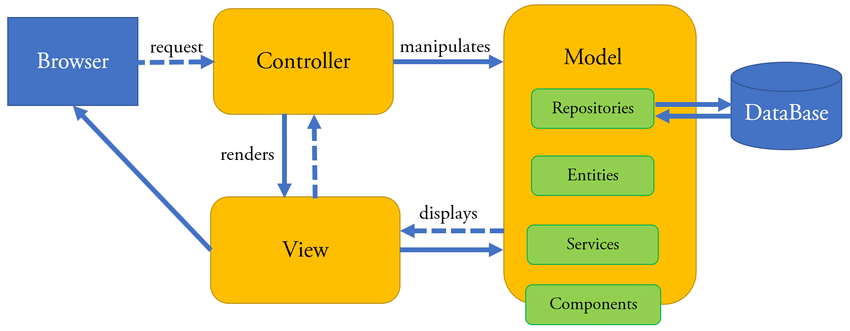
\includegraphics[width=0.85\textwidth]{mvc_architecture.png}
    \caption{MVC Architecture Model.}
    \label{fig:mvc_architecture}
\end{figure}

\subsection{Physical Architecture}
Physical architecture refers to the structure and layout of the physical components of an application.

The deployment diagram illustrates the architecture of a distributed application involving multiple components and services. The backend application contains the signaling controllers and routing logic, which communicate with the database for persistent storage. In parallel, an end user uses a PC on which a Next.js application runs via a web browser. The client utilizes WebSockets to communicate with the server and WebRTC to establish direct Peer-to-Peer (P2P) media connections with other clients. The different interactions between these components and services ensure the overall proper functioning of the application. The figure below presents the physical P2P coupling and signaling deployment flow of our application:

\begin{figure}[H]
    \centering
    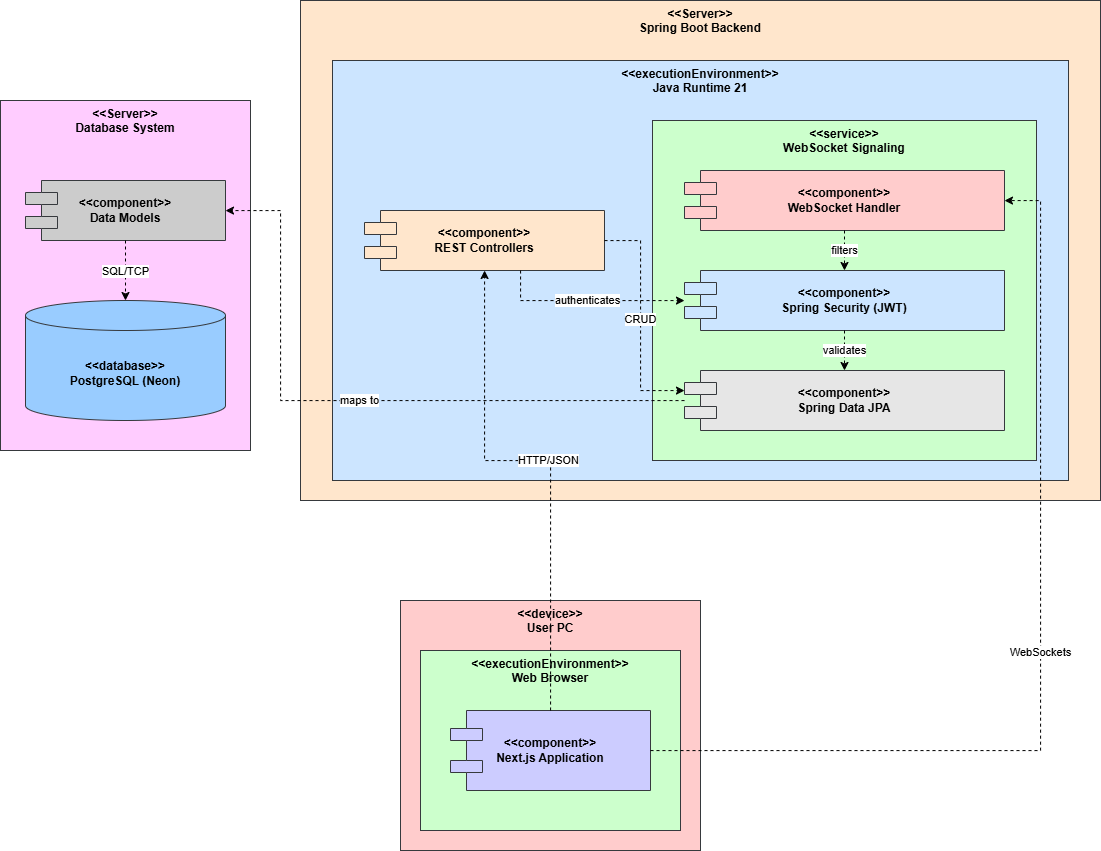
\includegraphics[width=\textwidth]{physical_architecture.png}
    \caption{Physical Component and Deployment Architecture.}
    \label{fig:physical_architecture}
\end{figure}

\section{Conclusion}
This chapter specified the user requirements, mapped security stories, detailed technology choices, and defined our core Zero-Knowledge architecture models. Chapter 3 details Release 1, focusing on authentication, key generation, and secure role isolation.